\chapter[Creating The Polar RZ Ensemble]{Creating The Polar RZ Ensemble}
\label{cp:creating-the-polar-rz-ensemble}

Nothing changed or to say here, we will just apply the same steps again.

\begin{listing} [!htpb]
    \caption{Creating the Polar RZ Ensemble.}
    \label{listing:PolarRZ-Ensemble}
    \begin{minted}{matlab}
%% Polar RZ
fprintf('\nPolar RZ\n');
pulse_RZ = [ones(1, floor(L/2)), zeros(1, ceil(L/2))];
ylim_RZ  = [-A-1, A+1];
color_RZ = [0.4940 0.1840 0.5560];

ensample_RZ = build_ensemble(data, A, pulse_RZ, N_realizations, L, 'polar');
    \end{minted}
\end{listing}

\begin{figure}[!htpb]
    \centering
    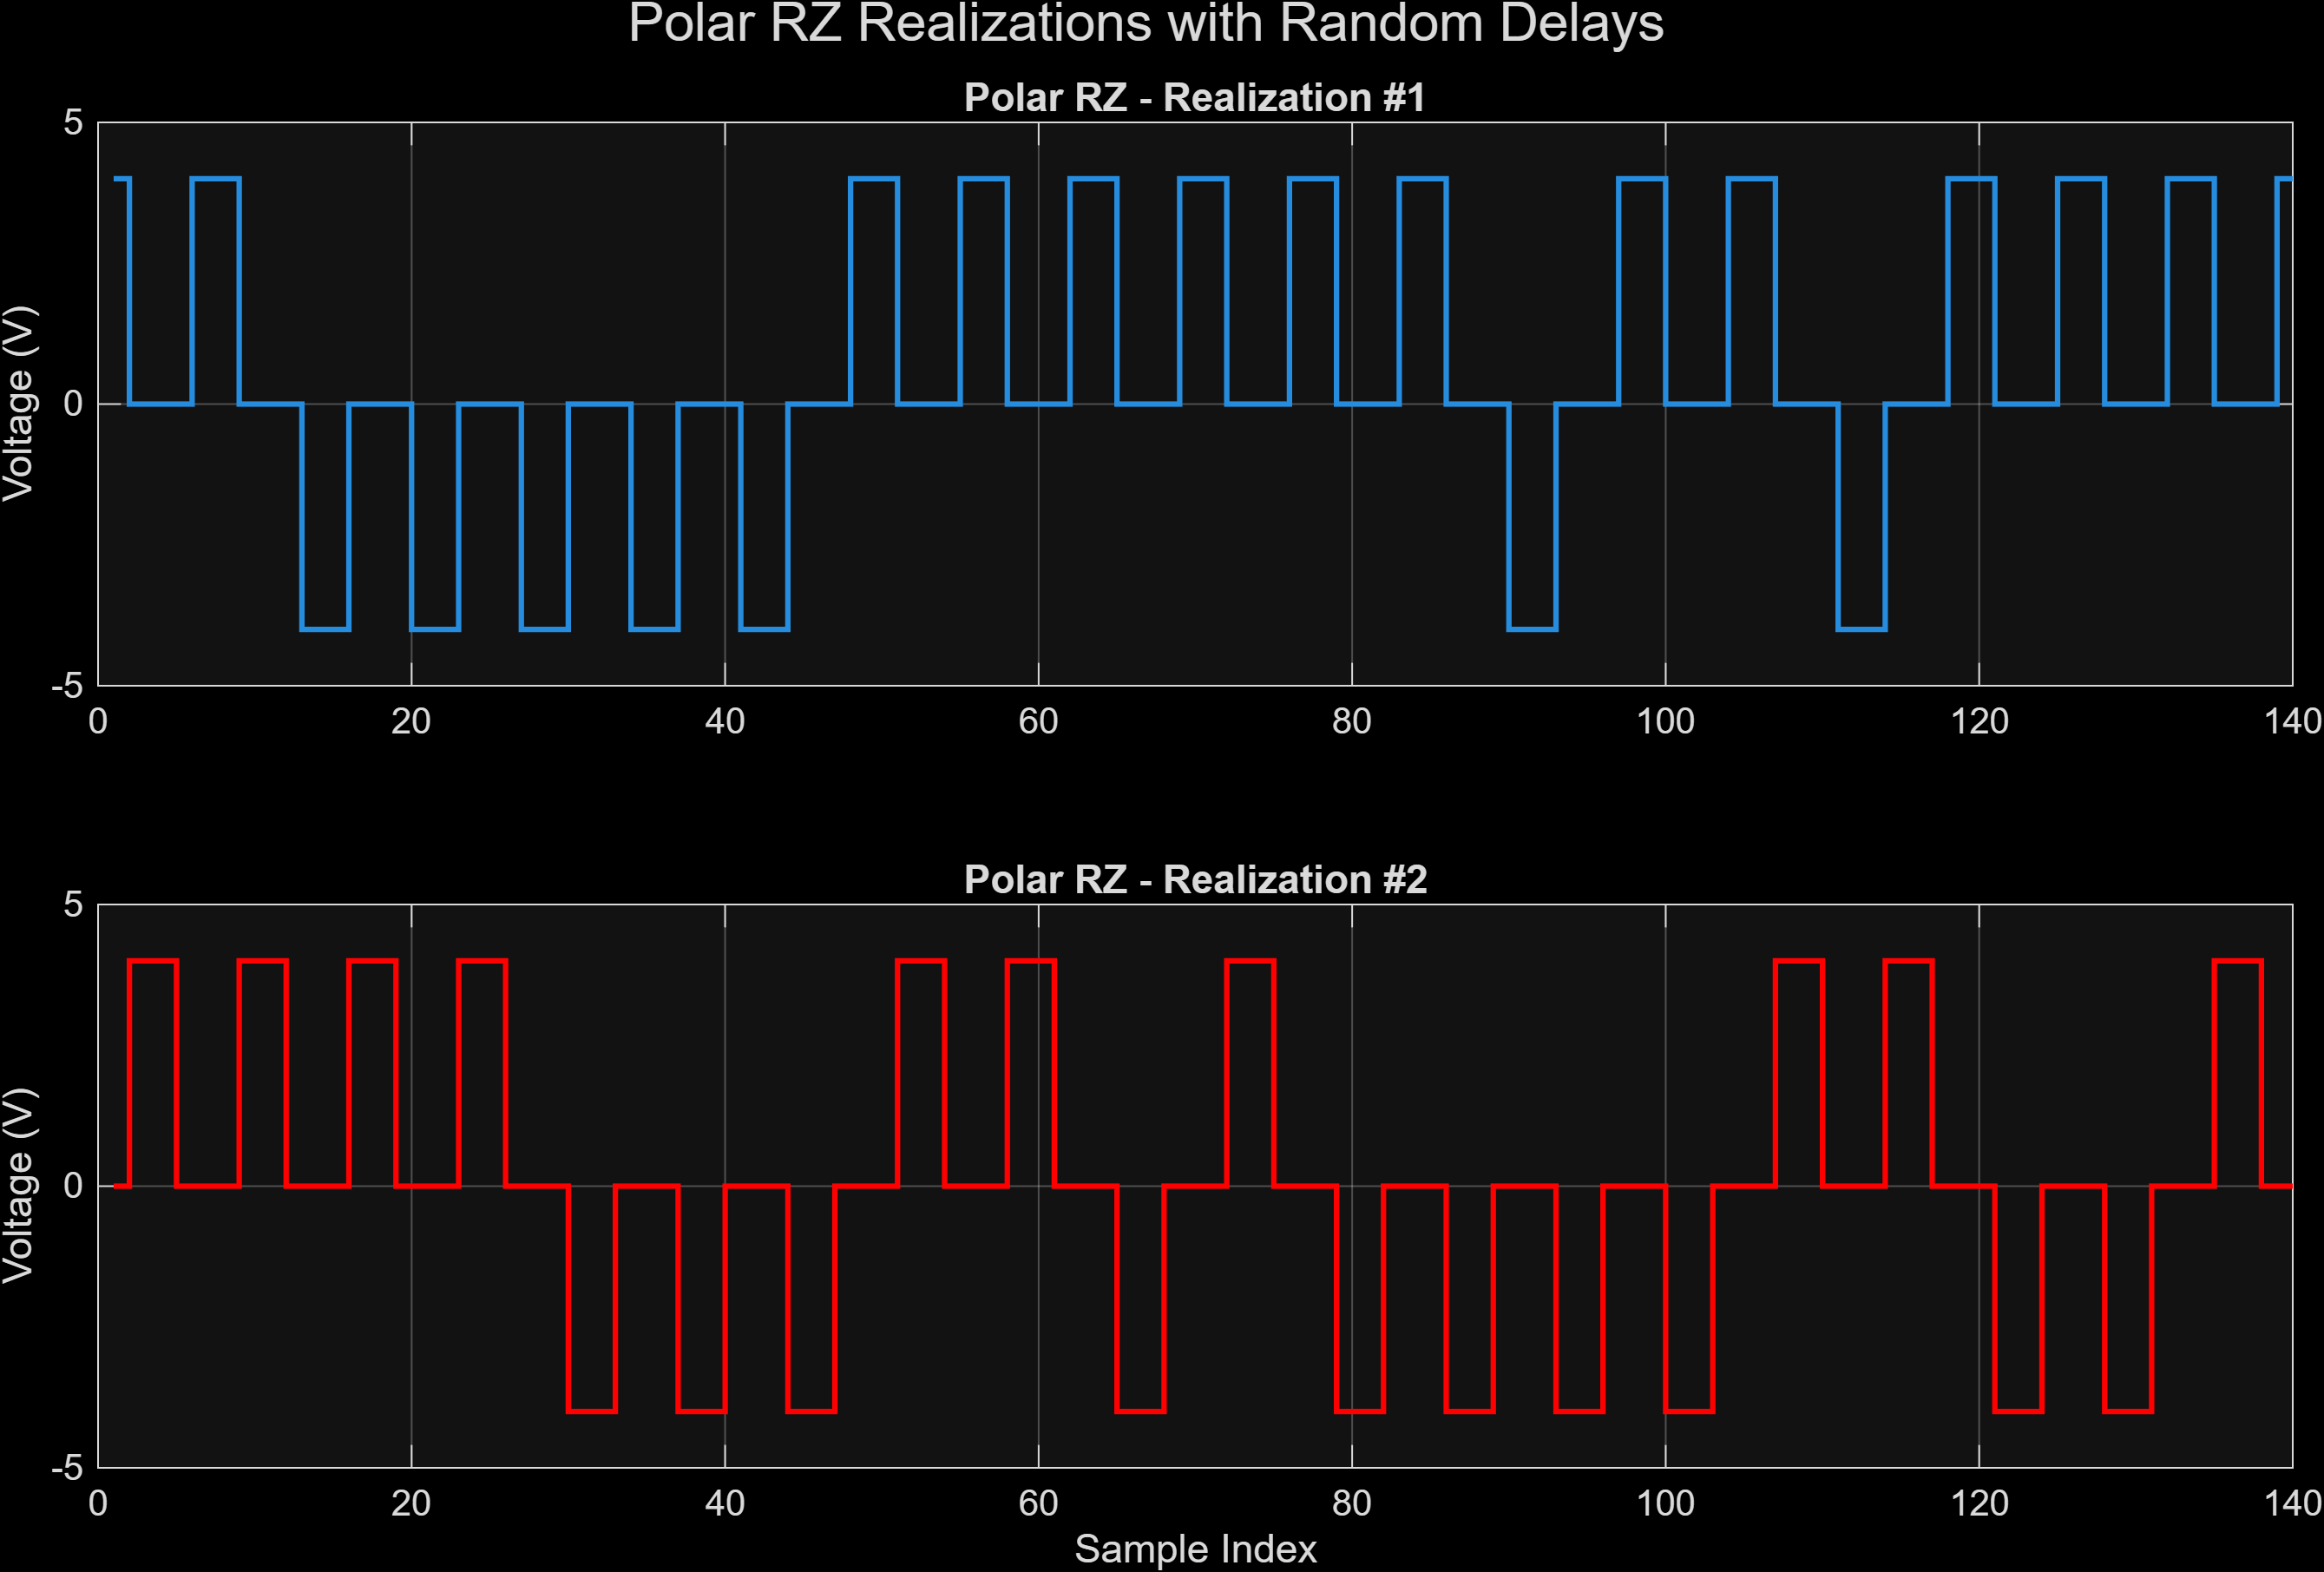
\includegraphics[width=0.75\linewidth]{Figures/Polar_RZ_-_Realization_2.png}
    \caption[Realization 1 and Realzation 2 from the Polar RZ Ensemble]{Realization 1 and Realzation 2 from the Polar RZ Ensemble.}
    \label{fig:POLAR-RZ-ENSEMBLE}
\end{figure}

As we can see in \autoref{fig:POLAR-RZ-ENSEMBLE}
\begin{itemize}
    \item The signal is now a pulse that lasts for half of the bit duration, and then goes to zero for the other half. This is the main characteristic of RZ signals.
    \item The pulse shape is rectangular, with a duration of $L$ samples per bit.
\end{itemize}